\chapter{Lec 11 - Unification and Generalized Modus Ponens}

\section{Problems with propositionalization}
The propositionalization approach is rather inefficient. For
example, given the query $Evil(x)$ and the knowledge base
\[
\begin{split}
    & \forall \, x \,\, King(x) \land Greedy(x) \Rightarrow Evil(x)\\
    & King(John)\\
    & Greedy(John)\\
    & Brother (Richard, John),
\end{split}
\]
it seems obvious the inference of $Evil(John)$, but propositionalization generates sentences such as $King(Richard) \land Greedy(Richard) \Rightarrow Evil(Richard)$ that are \textbf{irrelevant}. With $p$ k-ary predicates and $n$ constants, there are $p \cdot n^k$ instantiations!

\section{Unification}
The inference that John is evil, that is, that $\{x/John\}$ solves the query $Evil(x)$, works like this: to use the rule that greedy kings are evil, find some $x$ such that $x$ is a king and $x$ is
greedy, and then infer that this $x$ is evil.\newline\newline
More generally, if there is some substitution $\theta$ that makes each of the conjuncts of the premise of the implication identical to sentences already in the knowledge base, then we can assert the conclusion of the implication, after applying $\theta$. In this case, the substitution $\theta = \{x/John\}$ achieves that aim.\newline\newline
We can actually make the inference step do even more work. Suppose that instead of knowing $Greedy(John)$, we know that everyone is greedy:
\[\forall \, y \,\, Greedy(y)\]
Then we would still like to be able to conclude that $Evil(John)$.  In this case, applying the substitution $\{x/John, y/John\}$ to the implication premises $King(x)$ and $Greedy(x)$ and the knowledge-base sentences $King(John)$ and $Greedy(y)$ will make them identical. Thus, we can infer the conclusion of the implication.\newline\newline
This process is called \textbf{unification} and is a key component of all first-order inference algorithms. Unification finds a substitution that make different logical expressions look identical. The UNIFY algorithm takes two sentences and returns a unifier for them if one exists:
\begin{center}
    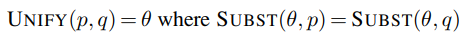
\includegraphics[]{images/unification.png}
\end{center}
Let us look at some examples of how UNIFY should behave. Suppose we have a query $AskVars(Knows(John, x))$: whom does John know? Answers to this query can be found by finding all sentences in the knowledge base that unify with $Knows(John, x)$. Here are the results of unification with four different sentences that might be in the knowledge base:
\begin{center}
    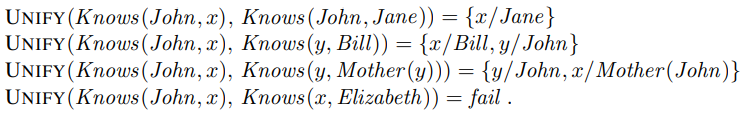
\includegraphics[]{images/unification ex.png}
\end{center}
The last unification fails because $x$ cannot take on the values $John$ and $Elizabeth$ at the same time. Now, remember that $Knows(x,Elizabeth)$ means \textit{“Everyone knows Elizabeth,”} so we should be able to infer that $John$ knows $Elizabeth$. The problem arises only because the two sentences happen to use the same variable name, $x$. The problem can be avoided by \textbf{standardizing apart} one of the two sentences being unified, which means renaming its variables to avoid name clashes. For example, we can rename $x$ in $Knows(x,Elizabeth)$ to $x_{17}$ (a new variable name) without changing its meaning. Now the unification will work:
\begin{center}
    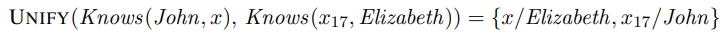
\includegraphics[]{images/standardizing-apart.png}
\end{center}
There is one more complication: we said that UNIFY should return a substitution that makes the two arguments look the same. But there could be more than one such unifier. For example, $UNIFY(Knows(John, x), Knows(y, z))$ could return $\{y/John, x/z\}$ or $\{y/John, x/John, z/John\}$. We say that the first unifier is more general than the second, because it places fewer restrictions on the values of the variables.  It turns out that, for every unifiable pair of expressions, there is a single \textbf{most general unifier} (or \textbf{MGU}) that is unique up to renaming and substitution of variables.
\begin{center}
    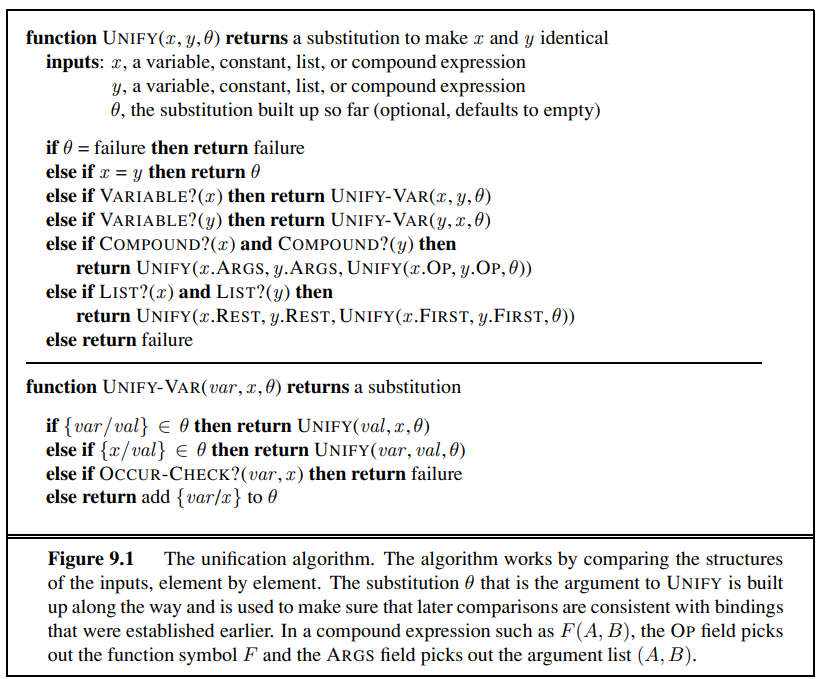
\includegraphics[]{images/unify-algo.png}
\end{center}
An algorithm for computing most general unifiers is shown in the figure above. The process is simple: recursively explore the two expressions simultaneously “side by side,” building up a unifier along the way, but failing if two corresponding points in the structures do not match. There is one expensive step: when matching a variable against a complex term, one must check whether the variable itself occurs inside the term; if it does, the match fails because no consistent unifier can be constructed. For example, $S(x)$ can’t unify with $S(S(x))$. This so called \textbf{occur check} makes the complexity of the entire algorithm quadratic in the size of the
expressions being unified.

\section{Generalized Modus Ponens (GMP)}
For atomic sentences $p_i$, $p'_i$ , and $q$, where there is a substitution $\theta$, such that $SUBST(\theta, p'_i ) = SUBST(\theta, p_i)$, for all $i$,
\begin{center}
    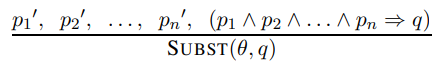
\includegraphics[]{images/GMP.png}
\end{center}
This inference rule is called \textbf{Generalized Modus Ponens} (\textbf{GMP}). There are $ n + 1$ premises to this rule: the $n$ atomic sentences $p'_i$ and the one implication. The
conclusion is the result of applying the substitution $\theta$ to the consequent $q$. For our example:
\begin{center}
    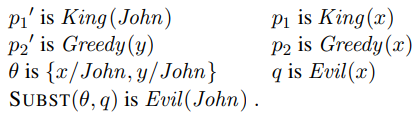
\includegraphics[]{images/GMP - Example.png}
\end{center}
Generalized Modus Ponens is a \textbf{sound} inference rule. We need to show that $p'_1, ..., p'_n, \, (p_1 \land ... \land p_n \Rightarrow q) \vDash Subst(\theta, q)$, provided that $Subst(\theta, p'_i) = Subst(\theta, p_i)$ for all $i$. First, we observe
that, for any sentence $p$ (whose variables are assumed to be universally quantified) and for any substitution $\theta$, 
\[p \vDash Subst(\theta, p)\]
holds by Universal Instantiation. It holds in particular for a $\theta$ that satisfies the conditions of the Generalized Modus Ponens rule. Thus, from $p'_1, ..., p'_n$ we can infer
\[Subst(\theta, p'_i) \land ... \land Subst(\theta, p'_n)\]
and from the implication $p_1 \land ... \land p_n \Rightarrow q$ we can infer
\[Subst(\theta, p_1) \land ... \land Subst(\theta, p_n) \Rightarrow Subst(\theta, q).
\]
Now, $\theta$ in Generalized Modus Ponens is defined so that $Subst(\theta, p'_i) = Subst(\theta, p_i)$, for all $i$; therefore the first of these two sentences matches the premise of the second exactly. Hence, $Subst(\theta, q)$ follows by Modus Ponens.

\section{First-order definite clauses}
A first order definite clause either is atomic or is an implication whose antecedent is a conjunction of positive literals and whose consequent is a single positive literal. Unlike propositional literals, first-order literals can include variables, in which case those variables are \textbf{assumed to be universally quantified}. (Typically, we omit universal quantifiers when writing definite clauses.) Consider the following problem:
\begin{center}
    "The law says that it is a crime for an American to sell weapons to hostile nations. The country Nono, an enemy of America, has some missiles, and all of its missiles were sold to it by Colonel West, who is American."
\end{center}
We will prove that West is a criminal. First, we will represent these facts as first-order definite clauses. The next section shows how the forward-chaining algorithm solves the problem.\newline\newline
“... it is a crime for an American to sell weapons to hostile nations”:
\begin{equation}
    American(x) \land Weapon(y) \land Sells(x, y, z) \land Hostile(z) \Rightarrow Criminal(x).
\end{equation}
“Nono ... has some missiles.” The sentence $\exists \, x \,\, Owns(Nono, x) \land Missile(x)$ is transformed into two definite clauses by Existential Instantiation, introducing a new constant $M_1$:
\begin{equation}
    Owns(Nono, M1) 
\end{equation}
\begin{equation}
    Missile(M1)
\end{equation}
"All of its missiles were sold to it by Colonel West”:
\begin{equation}
    Missile(x) \land Owns(Nono, x) \Rightarrow Sells(West, x, Nono).
\end{equation}
We will also need to know that missiles are weapons:
\begin{equation}
    Missile(x) \Rightarrow Weapon(x).
\end{equation}
and we must know that an enemy of America counts as “hostile”:
\begin{equation}
    Enemy(x, America) \Rightarrow Hostile(x).
\end{equation}
“West, who is American ...”:
\begin{equation}
    American(West)
\end{equation}
“The country Nono, an enemy of America ...”:
\begin{equation}
    Enemy(Nono, America)
\end{equation}
This knowledge base contains no function symbols and is therefore an instance of the class of \textbf{Datalog} knowledge bases. Datalog is a language that is restricted to first-order definite clauses with no function symbols. Datalog gets its name because it can represent the type of statements typically made in relational databases. We will see that the absence of function symbols makes inference much easier.

\section{Forward Chaining Algorithm}
The first forward-chaining algorithm we consider is a simple one. Starting from the known facts, it triggers all the rules whose premises are satisfied, adding their conclusions to the known facts. The process repeats until the query is answered (assuming that just one answer is required) or no new facts are added. We use our crime problem to illustrate how FOL-FC-ASK works. The implication
sentences are (1), (4), (5), (6). Two iterations are required:
\begin{itemize}
    \item On the first iteration, rule (1) has unsatisfied premises.
    \newline
    Rule (4) is satisfied with $\{x/M_1\}$, and $Sells(West, M_1, Nono)$ is added to the known facts. Note that Rule (4) is satisfied because the substitution  $\{x/M_1\}$ makes its premises equivalent to known facts in the KB.
    \newline
    Rule (5) is satisfied with $\{x/M_1\}$, and $Weapon(M_1)$ is added.
    \newline
    Rule (6) is satisfied with $\{x/Nono\}$, and $Hostile(Nono)$ is added.

    \item On the second iteration, rule (1) is satisfied with $\{x/West, y/M_1, z/Nono\}$, and $Criminal(West)$ is added.
\end{itemize}
\begin{center}
    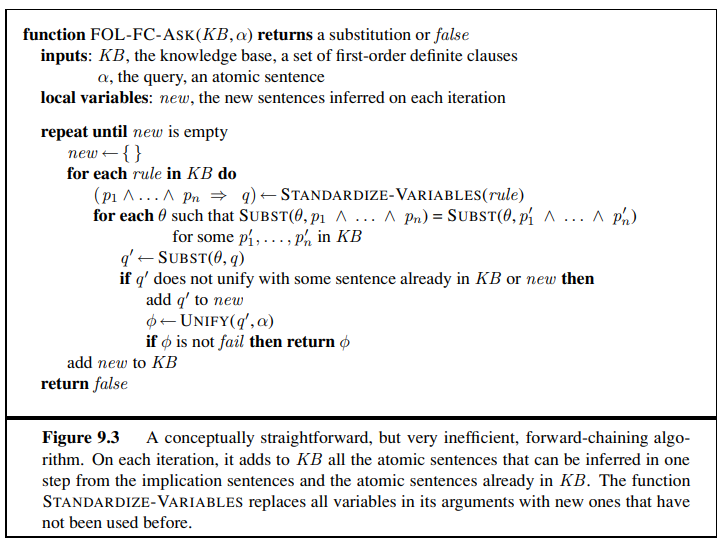
\includegraphics[]{images/FOL-FC.png}
    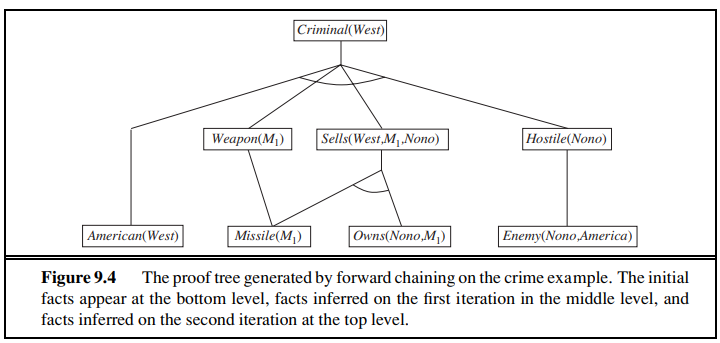
\includegraphics[]{images/FOL-FC proof tree.png}
\end{center}
Notice that no new inferences are possible at this point because every sentence that could be concluded by forward chaining is already
contained explicitly in the KB. Such a knowledge base is called a \textbf{fixed point} of the inference process.\newline\newline
Forward chaining is \textbf{sound}, because every inference is just an
application of Generalized Modus Ponens, which is sound. Second, it is \textbf{complete} for definite clause knowledge bases; that is, it answers every query whose answers are entailed by any knowledge base of definite clauses.\newline\newline
For Datalog knowledge bases, which contain no function symbols, forward chaining terminates in poly iterations. In fact, there can be no more than $pn^k$ distinct ground facts, where $k$ is  the maximum arity (number of arguments) of any predicate, $p$ be the number of predicates, and $n$ be the number of constant symbols.\newline\newline
For general definite clauses with function symbols, If the query has no answer, the algorithm could fail to terminate in some cases. This is unavoidable since entailment in first-order logic is semidecidable.

\subsection{Efficiency of forward chaining}
The forward-chaining algorithm shown in the figure above  is designed for ease of understanding rather than for efficiency of operation. There are three possible sources of inefficiency. First, the “inner loop” of the algorithm involves finding all possible unifiers such that the premise of a rule unifies with a suitable set of facts in the knowledge base. This is often called \textbf{pattern matching} and can be very expensive. Second, the algorithm rechecks every rule on every iteration to see whether its premises are satisfied, even if very few additions are made to the knowledge base on each iteration. Finally, the algorithm might generate many facts that are irrelevant to the goal.\newline\newline
The problem of matching the premise of a rule against the facts in the knowledge base might seem simple enough. However, it turns out that this problem is NP-Hard. Forward chaining can be extend to deal with these problems, but we will not see these extensions.
